\section{Desenvolvimento dos Osciladores em Anel}

Foram utilizadas as placas de desenvolvimento DE2 e ZedBoard. Elas foram escolhidas considerando suas disponibilidades no laboratório e por serem de fabricantes diferentes e possuírem nós tecnológicos diferentes.

A DE2 possui o FPGA XXXXX da família o Cyclone II da fabricante Altera, pertencente a Intel, que possui um nó tecnológico de 90nm. A Zedboard possui o FPGA YYYYYY, da Xilinx, agora pertencente a AMD, que possui um nó tecnológico de 28nm.

A topologia de oscilador em anel foi escolhida para os testes por sua disseminada utilização na caracterização de dispositivos MOSFET. Seu uso é amplo, pois medidas a utilizando se aproximam muito mais de aplicações reais do que medições paramétricas DC padrões.

Foram realizados testes preliminares com diferentes quantidades de inversores para encontrar uma quantidade apropriada, pois, com poucos osciladores não há tempo suficiente para os inversores chavearem e com muitos osciladores o limite de iterações que as IDEs permitem era atingido.

Considerando isso, foi decidido que em cada um dos dispositivos foi sintetizado dois osciladores, um com 1001 inversores e outro com 4999. A escolha de utilizar dois osciladores em cada FPGA foi tomada por dois motivos: para se ter certeza que as IDEs não estavam simplificando os estágios inversores do circuito sintetizado e para verificar que o envelhecimento afeta igualmente diferentes partes do FPGA.

A grande quantidade de inversores é relevante, pois assim as pequenas variações aleatórias nas características de cada transistor que compõe os dispositivos tenderão a se diluir.

\subsection{Desenvolvimento do Código para os Osciladores}

Para desenvolver e sintetizar os osciladores em anel foi utilizada a linguagem de descrição Verilog. Para o Cyclone II foi utilizada a IDE Quartus II versão 12.1, já para o ZedBoard foi utilizada a IDE Vivado versão 2023.1.

O Quadro \ref{code:RingOsc} mostra o código desenvolvido em Verilog para o módulo que implementa o oscilador em anel com N inversores. O mesmo código foi utilizado para os dois FPGAs nas duas IDEs diferentes.

\begin{lstlisting}[label={code:RingOsc}, style=VerilogStyle, caption={Módulo do Oscilador em Anel. Fonte: O Autor}]
module RingOscillator 
	#(parameter N = 5)
	(
		input  en,
		output reg and_1    /*synthesis keep*/
	);
	reg [N - 1:0] notGate /*synthesis keep*/;
	integer i;
	generate
	  always @ (*) begin
		  and_1 <= en & notGate[N - 1];
	  	notGate[0] <= ~and_1;
	  	for (i = 1; i < N; i = i + 1)   begin: inverter_chain
			  notGate[i] <= ~notGate[i - 1];
		  end
	  end
	endgenerate
endmodule
\end{lstlisting}

O módulo possui uma entrada en, responsável por habilitar o circuito, uma saída and\_1 que é a saída da porta and do circuito, de onde o sinal do oscilador é obtido. O valor N é parametrizável, o que permite a reutilização do mesmo código para osciladores com diferentes números de inversores.

São então instanciadas N registradores, que serão utilizados para criar os inversores. O registrador and\_1 recebe o resultado da operação E lógica do sinal de enable e a saída do último inversor. O primeiro inversor é definido como o registrador and\_1 invertido.

Um bloco 'for' é utilizado para automatizar as atribuições dos inversores seguintes, sendo a cada um atribuído o valor inversor anterior negado.

Um ponto importante de destacar é a necessidade de utilizar diretivas de compilação para impedir que os inversores sejam simplificados na síntese. Essas diretivas são diferentes em cada uma das IDEs, na Quartus II é utilizado a diretiva /* synthesis keep */ e na Vivado é utilizado a diretiva /* synthesis syn\_keep=1 */.

Na Figura \ref{fig:DE2Imp3Osc} pode ser visto como o Quartus II implementa em hardware o código do Quadro \ref{code:RingOsc} para um N igual a 3. A implementação é feita através de portas lógicas comuns, o que é diferente da implementação feita pelo Vivado, como visto na FIgura \ref{fig:ZedImp3Osc}, que utiliza LUTs de uma variável para representar os inversores.

\begin{figure}[H]
    \centering
    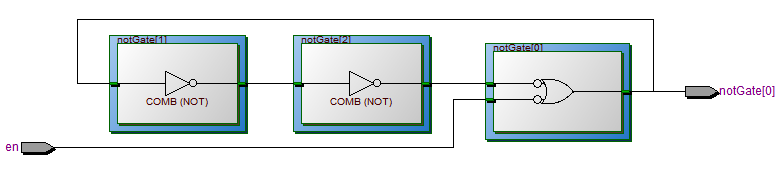
\includegraphics[width=\linewidth]{figures/DE2_Implementation_3Inverter_Gates.png}
    \caption{Síntese do módulo de alto nível gerado no Quatus II. Fonte: O Autor}
    \label{fig:DE2Imp3Osc}
\end{figure}

\begin{figure}[H]
    \centering
    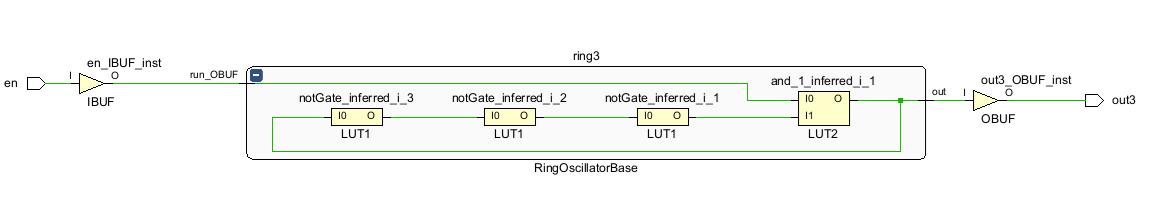
\includegraphics[width=\linewidth]{figures/ZedBoard_Implementation_3Inverter.png}
    \caption{Síntese do módulo de alto nível gerado no Vivado. Fonte: O Autor}
    \label{fig:ZedImp3Osc}
\end{figure}

O Quadro \ref{code:TopLevel} mostra o módulo de alto nível em que é instanciado dois osciladores em anel, um com 1001 e outro de 4999 inversores. 

\begin{lstlisting}[label={code:TopLevel}, style=VerilogStyle, caption={Estanciamento dos Módulos. Fonte: O Autor}]
module TopLevel
	(
		input en,
		output run,
		output out1001, out4999
	);
	
	assign run = en;

	RingOscillator #(.N(1001)) ring1001(en, out1001);
	RingOscillator #(.N(4999)) ring4999(en, out4999);
endmodule
\end{lstlisting}

O módulo possui uma entrada en, responsável por habilitar o circuito, uma saída run, usada para indicar que o circuito está em funcionamento e as saídas dos dois osciladores out1001, out4999. Também são declaradas duas instâncias do módulo desenvolvido no Quadro \ref{code:RingOsc}.

As Figuras \ref{fig:DE2RtlSchem} e \ref{fig:ZedRtlSchem1} mostram, respectivamente, o circuito implementado pelo software Quartus II e Vivado para o módulo de alto nível que serão utilizado nos FPGAs.

\begin{figure}[H]
    \centering
    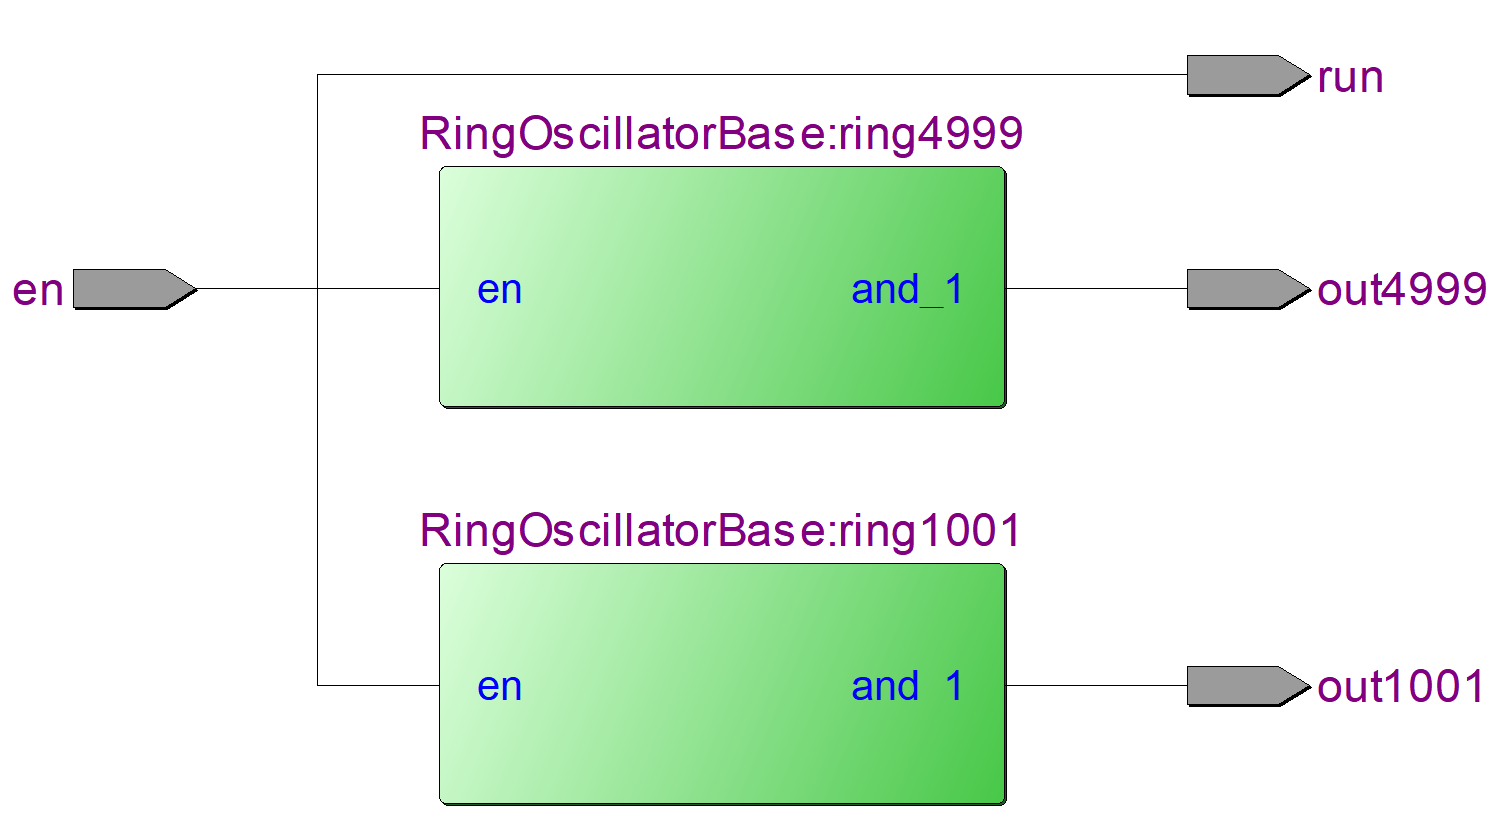
\includegraphics[scale=0.25]{figures/DE2_RTL_Schematic.png}
    \caption{Síntese de um oscilador com três inversores gerado no Quatus II. Fonte: O Autor}
    \label{fig:DE2RtlSchem}
\end{figure}

\begin{figure}[H]
    \centering
    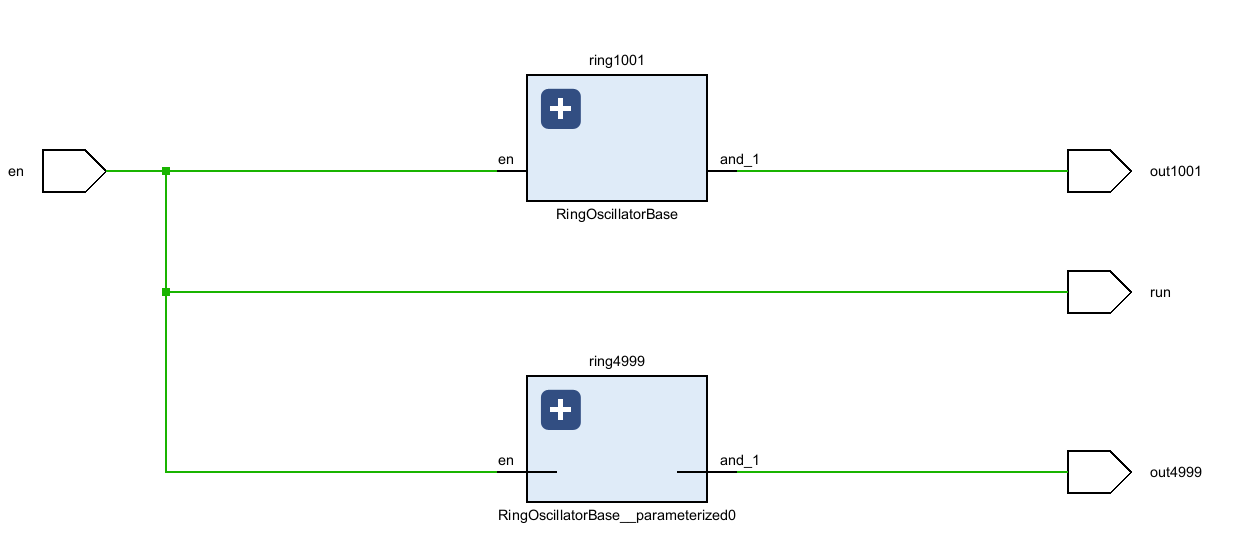
\includegraphics[width=\linewidth]{figures/ZedBoard_RTL_Schematic.png}
    \caption{Síntese de um oscilador com três inversores gerado no Vivado. Fonte: O Autor}
    \label{fig:ZedRtlSchem1}
\end{figure}

Após o desenvolvimento, o circuito sintetizado foi simulado utilizando a ferramenta apropriada para cada um dos componentes. Constatada a validade da solução ela foi transferida para os FPGAs reais e será medida, através de um osciloscópio, a frequência de oscilação das saídas do circuitos.